\documentclass[margin=1cm,varwidth]{standalone}
\usepackage{feynman-diagram}


\begin{document}
\begin{tikzpicture}
  \firstvertex{V1}{-135,135,0}{f,F,B}[\(e^-\),\(e^+\),\(\gamma\)]
              [1.15,1.15,0.5][midway,midway,above]
  \vertex{V2}{V1}{3}{-45,45}{F,f}[\(e^-\), \(e^+\)]
\end{tikzpicture}

\end{document}
